\documentclass[tikz]{standalone}
\usetikzlibrary{chains,shadows.blur}
% For decorating a path with text.
\begin{document}

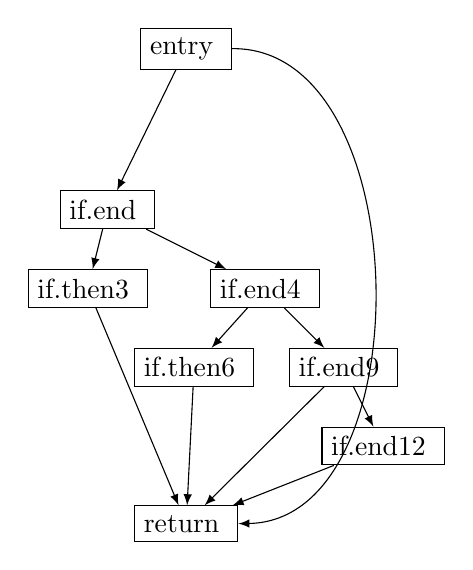
\begin{tikzpicture}[node distance = 8mm, start chain = going below, box/.style = {draw,rounded corners, on chain, align=center}]
\node[box, sharp corners] (entry) at (2, -0.00) { entry };
\node[box, sharp corners] (if_end) at (1, -1.00) { if.end };
\node[box, sharp corners] (if_then3) at (0.75, -2.00) { if.then3 };
\node[box, sharp corners] (if_end4) at (3, -2.00) { if.end4 };
\node[box, sharp corners] (if_then6) at (2.1, -3.00) { if.then6 };
\node[box, sharp corners] (if_end9) at (4, -3.00) { if.end9 };
\node[box, sharp corners] (if_end12) at (4.50, -4.00) { if.end12 };
\node[box, sharp corners] (return) at (2, -5.00) { return };

\begin{scope}[rounded corners,-latex]
\path [color=black] (entry) edge[ bend left=0 ] (if_end);
\path [color=black] (entry) edge[ bend left=90 ] (return);
\path [color=black] (if_end) edge[ bend left=0 ] (if_end4);
\path [color=black] (if_end) edge[ bend left=0 ] (if_then3);
\path [color=black] (if_then3) edge[ bend left=0 ] (return);
\path [color=black] (if_end4) edge[ bend left=0 ] (if_end9);
\path [color=black] (if_end4) edge[ bend left=0 ] (if_then6);
\path [color=black] (if_then6) edge[ bend left=0 ] (return);
\path [color=black] (if_end9) edge[ bend left=0 ] (if_end12);
\path [color=black] (if_end9) edge[ bend left=0 ] (return);
\path [color=black] (if_end12) edge[ bend left=0 ] (return);
\end{scope}
\end{tikzpicture}

\end{document}
